\documentclass[aspectratio=169]{beamer}

\mode<presentation>
{
  \usetheme{Spil}
  \setbeamercovered{invisible}
}

\usepackage[english]{babel}
\usepackage[latin1]{inputenc}

\usepackage{times}
\usepackage[T1]{fontenc}

% Anchoring images
%\usepackage[absolute, overlay]{textpos}

\title[]{\alert{Spilgames Storage Platform}}

\author[]{Enrique Paz}
%\author{\texorpdfstring{Author\newline\url{email@email.com}}{Author}}

\institute[] % (optional, but mostly needed)
{Senior Backend Developer}

\date[]{21/03/2013}

\AtBeginSection[]{
    \begin{frame}
        \begin{center}
            \huge{\insertsectionhead}
        \end{center}
    \end{frame}
}

\begin{document}

\begin{frame}
    \titlepage
\end{frame}

\section{Introduction}
\subsection{Spilgames \& Me}

\begin{frame}{About Me}
    \begin{columns}
        \begin{column}[c]{0.05\textwidth}
        \end{column}
        \begin{column}[c]{0.2\textwidth}
            \includegraphics[width=\textwidth]{images/me.png}
        \end{column}
        \begin{column}[c]{0.05\textwidth}
        \end{column}
        \begin{column}[c]{0.7\textwidth}
            \begin{itemize}
                \item Passionate Erlang Developer
                \item Testing Enthusiast
                \item Development Process Caretaker
                % \item Triumph Rider
                % TODO Picture with the bike
            \end{itemize}
        \end{column}
    \end{columns}
\end{frame}

\begin{frame}{Spilgames}
    \begin{itemize}
       \item Gaming Platform
       \item Serving data to 190+ countries world-wide
       \item 180+ million unique users per month
       \item Multiple Platforms: Desktop, Mobile Native \& Web
       \item 300+ employees
       \item Offices in The Netherlands \& China
       \item Revenue: Advertising \& EUM
    \end{itemize}
\end{frame}

\begin{frame}{Gaming Portals}
    \includegraphics[width=\textwidth]{images/gamesgames.png}
\end{frame}

\begin{frame}{Gaming Portals}
    \includegraphics[width=\textwidth]{images/ggg.png}
\end{frame}

\begin{frame}{Games}
    \begin{columns}
        \begin{column}[c]{0.5\textwidth}
            \includegraphics[height=0.6\textheight]{images/sarah.png}
        \end{column}
        \begin{column}[c]{0.5\textwidth}
            \includegraphics[height=0.6\textheight]{images/galaxylife.png}
        \end{column}
    \end{columns}
\end{frame}

\section{Another Storage}

{
\usebackgroundtemplate{\includegraphics[width=\paperwidth]{images/anotherstorage.png}}
\begin{frame}{Another Storage}
\end{frame}
}

\subsection{Motivation}

\begin{frame}{LAMP Stack \& MySql}
    \begin{itemize}
        \item Not all developers are DB experts
        \item Difficult to shard the databases
        \item Security
        \item Performance
        \item Caching
        \item \dots
    \end{itemize}
\end{frame}

\begin{frame}{Our Ambition}
    \begin{columns}
        \begin{column}[c]{0.1\textwidth}
        \end{column}
        \begin{column}[c]{0.9\textwidth}
            \includegraphics[width=0.8\textwidth]{images/storageusage.png}
        \end{column}
    \end{columns}
\end{frame}

\begin{frame}{Wish List}
    \begin{itemize}
        \item Transparent sharding layer
        \item Scalable applications on top of sharding data
        \item High Availability
        \item Centralized caching layer
        \item Storage engine agnostic
        \item Allow changes to storage layer without affecting business (versioning)
        \item Ability to scale geographically
    \end{itemize}
\end{frame}

\begin{frame}{One API to rule them All}
    \begin{itemize}
        \item ``Don't care where it is, just want my data!!!''
        \pause
        \begin{columns}
            \begin{column}[c]{0.55\textwidth}
                    \begin{itemize}
                        \item \href{http://piqi.org}{PIQI}
                        \item Native erlang (+ Protocol Buffers)
                        \item HTTP + JSON
                        \item HTTP + Protocol Buffers
                    \end{itemize}
            \end{column}
            \begin{column}[c]{0.45\textwidth}
                \includegraphics[width=\textwidth]{images/piqi.png}
            \end{column}
        \end{columns}
    \end{itemize}
\end{frame}

\section{System Properties}

\subsection{Overview}

\begin{frame}{Mindset}
    \begin{itemize}
        \item Always available
        \item No global locks
        \item Inconsistencies are the norm
            \begin{itemize}
                \item Hardware breaks down (power failures)
                \item Version mismatches (upgrading system not atomic)
                \item State mismatches (adding new machines)
            \end{itemize}
    \end{itemize}
\end{frame}

\begin{frame}{A Key-Value Store With Schema}
    \begin{itemize}
        \item \textbf{Buckets}:
            \begin{itemize}
                \item Are largely generated OTP applications
                \item Expose a clear interface
            \end{itemize}
        \item All data is identified by a \textbf{GID}
        \item GID types for data owners: users \& games
        \item Buckets can use different data storage engines:
            \begin{itemize}
                \item Several MySql tables in different databases
                \item Just a binary storage (SWIFT)
                \item \dots
            \end{itemize}
    \end{itemize}
\end{frame}

\begin{frame}{A Key-Value Store With Schema}
    \begin{itemize}
        \item Buckets offer a CRUD-like interface (with filters)
        \item All data for a bucket/GID is cached locally
        \item Requests are atomic per bucket/GID combination
    \end{itemize}
\end{frame}

\begin{frame}{Optimistic Operations}
    \begin{itemize}
        \item Speed > Consistency
        \item Losing some updates is case of crash is affordable
        \item Destructive operations act first on cache and eventually on disk
        \item No warranties of eventual consistency upon crashes
            \begin{itemize}
                \item i.e. Activity feeds
                \item i.e. Popular Games List
            \end{itemize}
    \end{itemize}
\end{frame}

\begin{frame}{Pessimistic Operations}
    \begin{itemize}
        \item Consistency is key and confirmation is required
        \item Dealing with critical data
        \item Destructive operations act on disk and, upon success, on cache
            \begin{itemize}
                \item i.e. Payments
                \item i.e. Personal Information
            \end{itemize}
    \end{itemize}
\end{frame}

\subsection{Internals}
{
\usebackgroundtemplate{\includegraphics[height=\paperheight]{images/howitworks.png}}
\begin{frame}{How does it work?}
\end{frame}
}

\begin{frame}{System Components}
    % XXX Maybe picture of the ring?
    \begin{itemize}
        \item The \textbf{lookup} application must run in every SSP node
        \item A \textbf{hashing ring} relates GID ranges with \textbf{pipeline factory} (PF) PIDs
        \item Buckets in a node register in the lookup application
        \item There can be several PFs per bucket/node
        \item The hashing ring is a distributed mnesia table:
            \begin{itemize}
                \item ram\_copies
                \item dirty reads
                \item transactional writes
            \end{itemize}
    \end{itemize}
\end{frame}

\begin{frame}{Tracing Pessimistic Operations}
    \begin{enumerate}
        \item A random SSP node receives a request for a bucket/GID
        \item The node uses the lookup service to locate a PF at any node
        \item The requested operation is encoded by the remote PF
        \item The remote PF queues the operation in a pipeline for the given GID
    \end{enumerate}
\end{frame}

\begin{frame}{A Closer Look}
% TODO Sequence diagram overview of system behavior (pessimistic insert)
\end{frame}

\begin{frame}{Wait a minute\dots}
    \begin{columns}
        \begin{column}[c]{0.05\textwidth}
        \end{column}
        \begin{column}[c]{0.3\textwidth}
            \includegraphics[width=\textwidth]{images/slow.png}
        \end{column}
        \begin{column}[c]{0.65\textwidth}
            \begin{itemize}
                \item ``Why do we need pipelines?''
                \item ``Sequential == Bottleneck !!!''
                \item ``Don't you guys know Erlang is about \textbf{parallelizing} work?''
            \end{itemize}
        \end{column}
    \end{columns}
\end{frame}

\begin{frame}{About Pipelines}
    \begin{itemize}
        \item Drawbacks
            \begin{itemize}
                \item For hotspots sequential (read) access is bad indeed.\\
                    i.e. Retrieving game data for popular games
                \item Optimization: read from cache outside the pipeline
            \end{itemize}
        \pause
        \item Advantages
            \begin{itemize}
                \item Scales without global locks
                \item Easy multi-database consistency
            \end{itemize}
        \pause
        \item Requests to most GIDs (users) are evenly distributed
    \end{itemize}
\end{frame}

\subsection{Versions, Shards \& Migration}

\begin{frame}{Schema Versions}
    \begin{itemize}
        \item A bucket is versioned
        \item Schema Versions determine allowed operations and storage(s)
        \item 1 or 2 versions of a bucket are allowed at the time
    \end{itemize}
\end{frame}

\begin{frame}{Shards}
    \begin{itemize}
        \item Useful for partitioning big blocks of data
        \item Sharding rules are bucket specific. Default is GID \% Shards
        \item SSP stores and caches versions and shards information internally
    \end{itemize}
\end{frame}

\begin{frame}{Working With Versions \& Shards}
    \begin{table}{
        \small
        \begin{tabular}{|l|l|l|l|l|l|}
            \hline
            \textbf{Bucket}&\textbf{GID}&\textbf{Version}&\textbf{Shard}&\textbf{Mirror}&\textbf{Previous}\\
            \hline
            profile&288234639967094968&1&3&1&0\\
            \dots&\dots&\dots&\dots&\dots&\dots\\
            \hline
        \end{tabular}}
    \end{table}
    \begin{columns}
        \begin{column}[c]{0.33\textwidth}
            \begin{itemize}
                \item Migrations
            \end{itemize}
        \end{column}
        \begin{column}[c]{0.33\textwidth}
            \begin{itemize}
                \item Read Previous
            \end{itemize}
        \end{column}
        \begin{column}[c]{0.33\textwidth}
            \begin{itemize}
                \item Mirror Write
            \end{itemize}
        \end{column}
    \end{columns}
\end{frame}

\section{Worldwide}

{
\usebackgroundtemplate{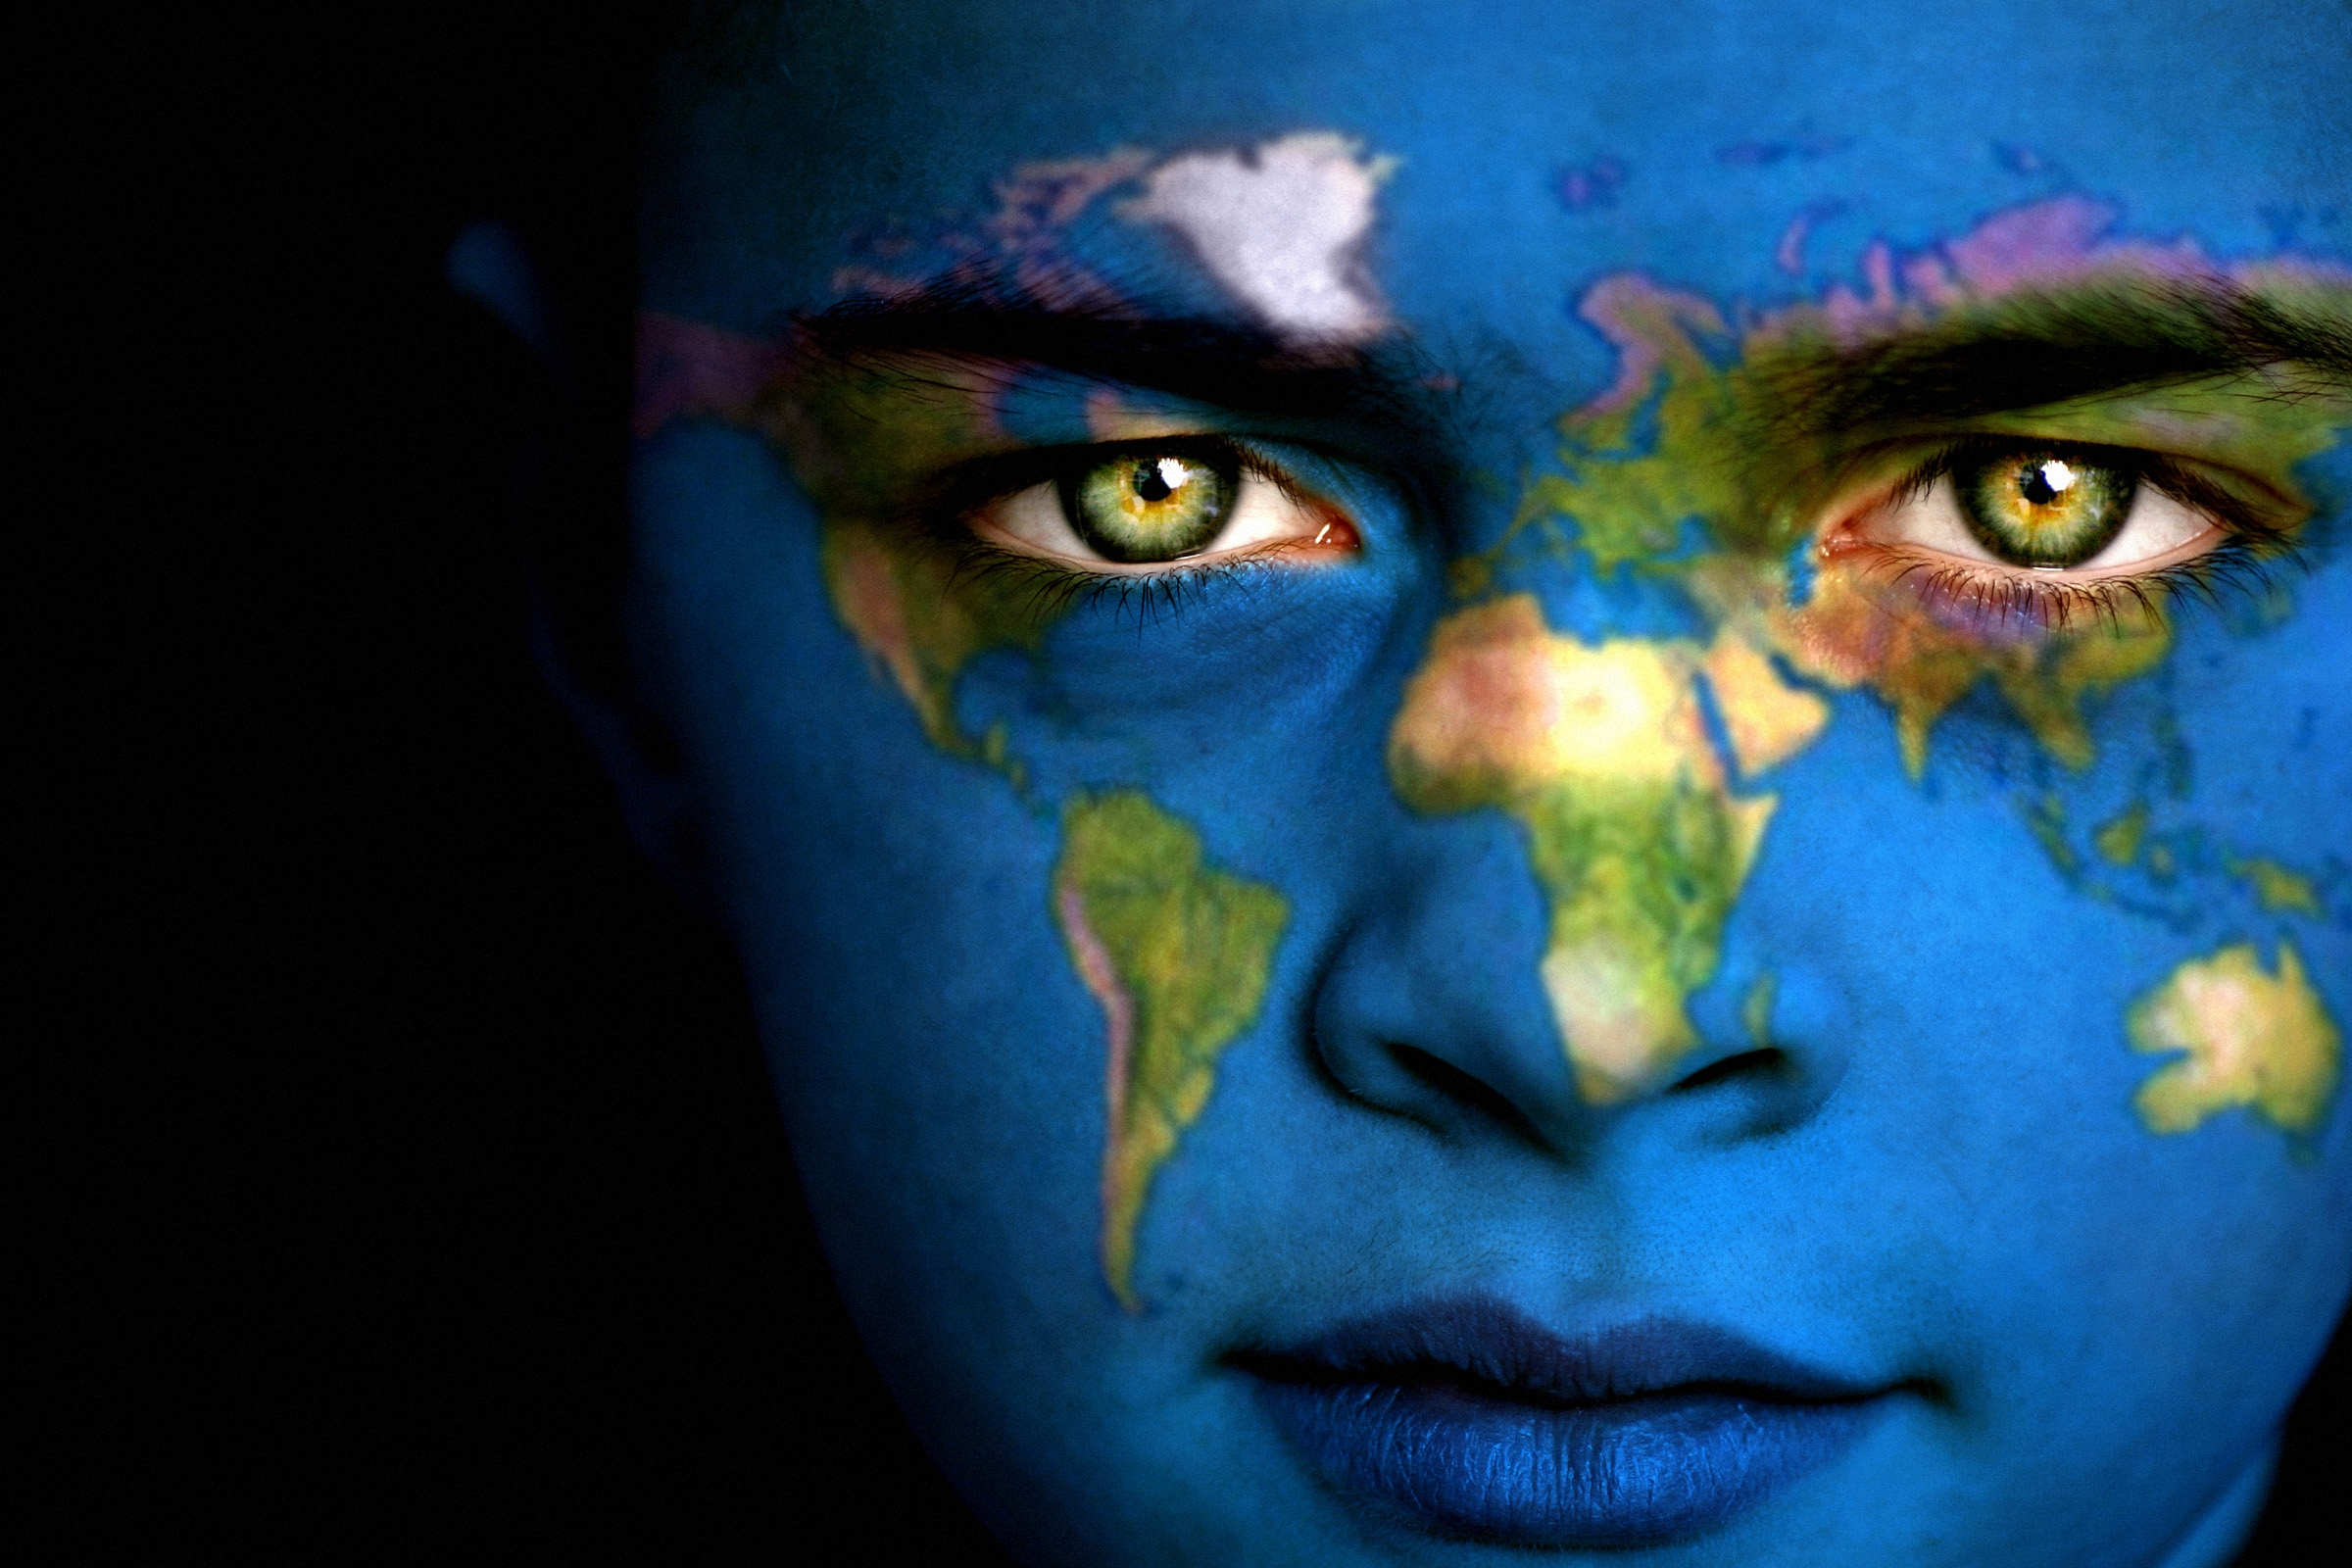
\includegraphics[width=\paperwidth]{images/worldwide.png}}
\begin{frame}{Worlwide}
\end{frame}
}

\subsection{Scaling Datacenters}

\begin{frame}{Operating Globally}
    \begin{center}
        \includegraphics[width=0.7\textwidth]{images/worldmapdc.png}
    \end{center}
\end{frame}

\begin{frame}{Working With Multiple Datacenters}
    \begin{columns}
        \begin{column}[c]{0.1\textwidth}
        \end{column}
        \begin{column}[c]{0.8\textwidth}
            \includegraphics[width=0.8\textwidth]{images/multidcops.png}
        \end{column}
        \begin{column}[c]{0.1\textwidth}
        \end{column}
    \end{columns}
\end{frame}

\begin{frame}{Masters \& Satellites}
    \begin{itemize}
        \item Master Datacenters
            \begin{itemize}
                \item Have persistent storage
                \item Can own GIDs
                \item GIDs ownership can be migrated from one Master DC to another
            \end{itemize}
        \pause
        \item Satellite Datacenters
            \begin{itemize}
                \item Can't own GIDs
                \item Don't have persistent storage
                \item Easy to setup and decommission
            \end{itemize}
    \end{itemize}
\end{frame}

\subsection{Disaster Scenarios}

{
\usebackgroundtemplate{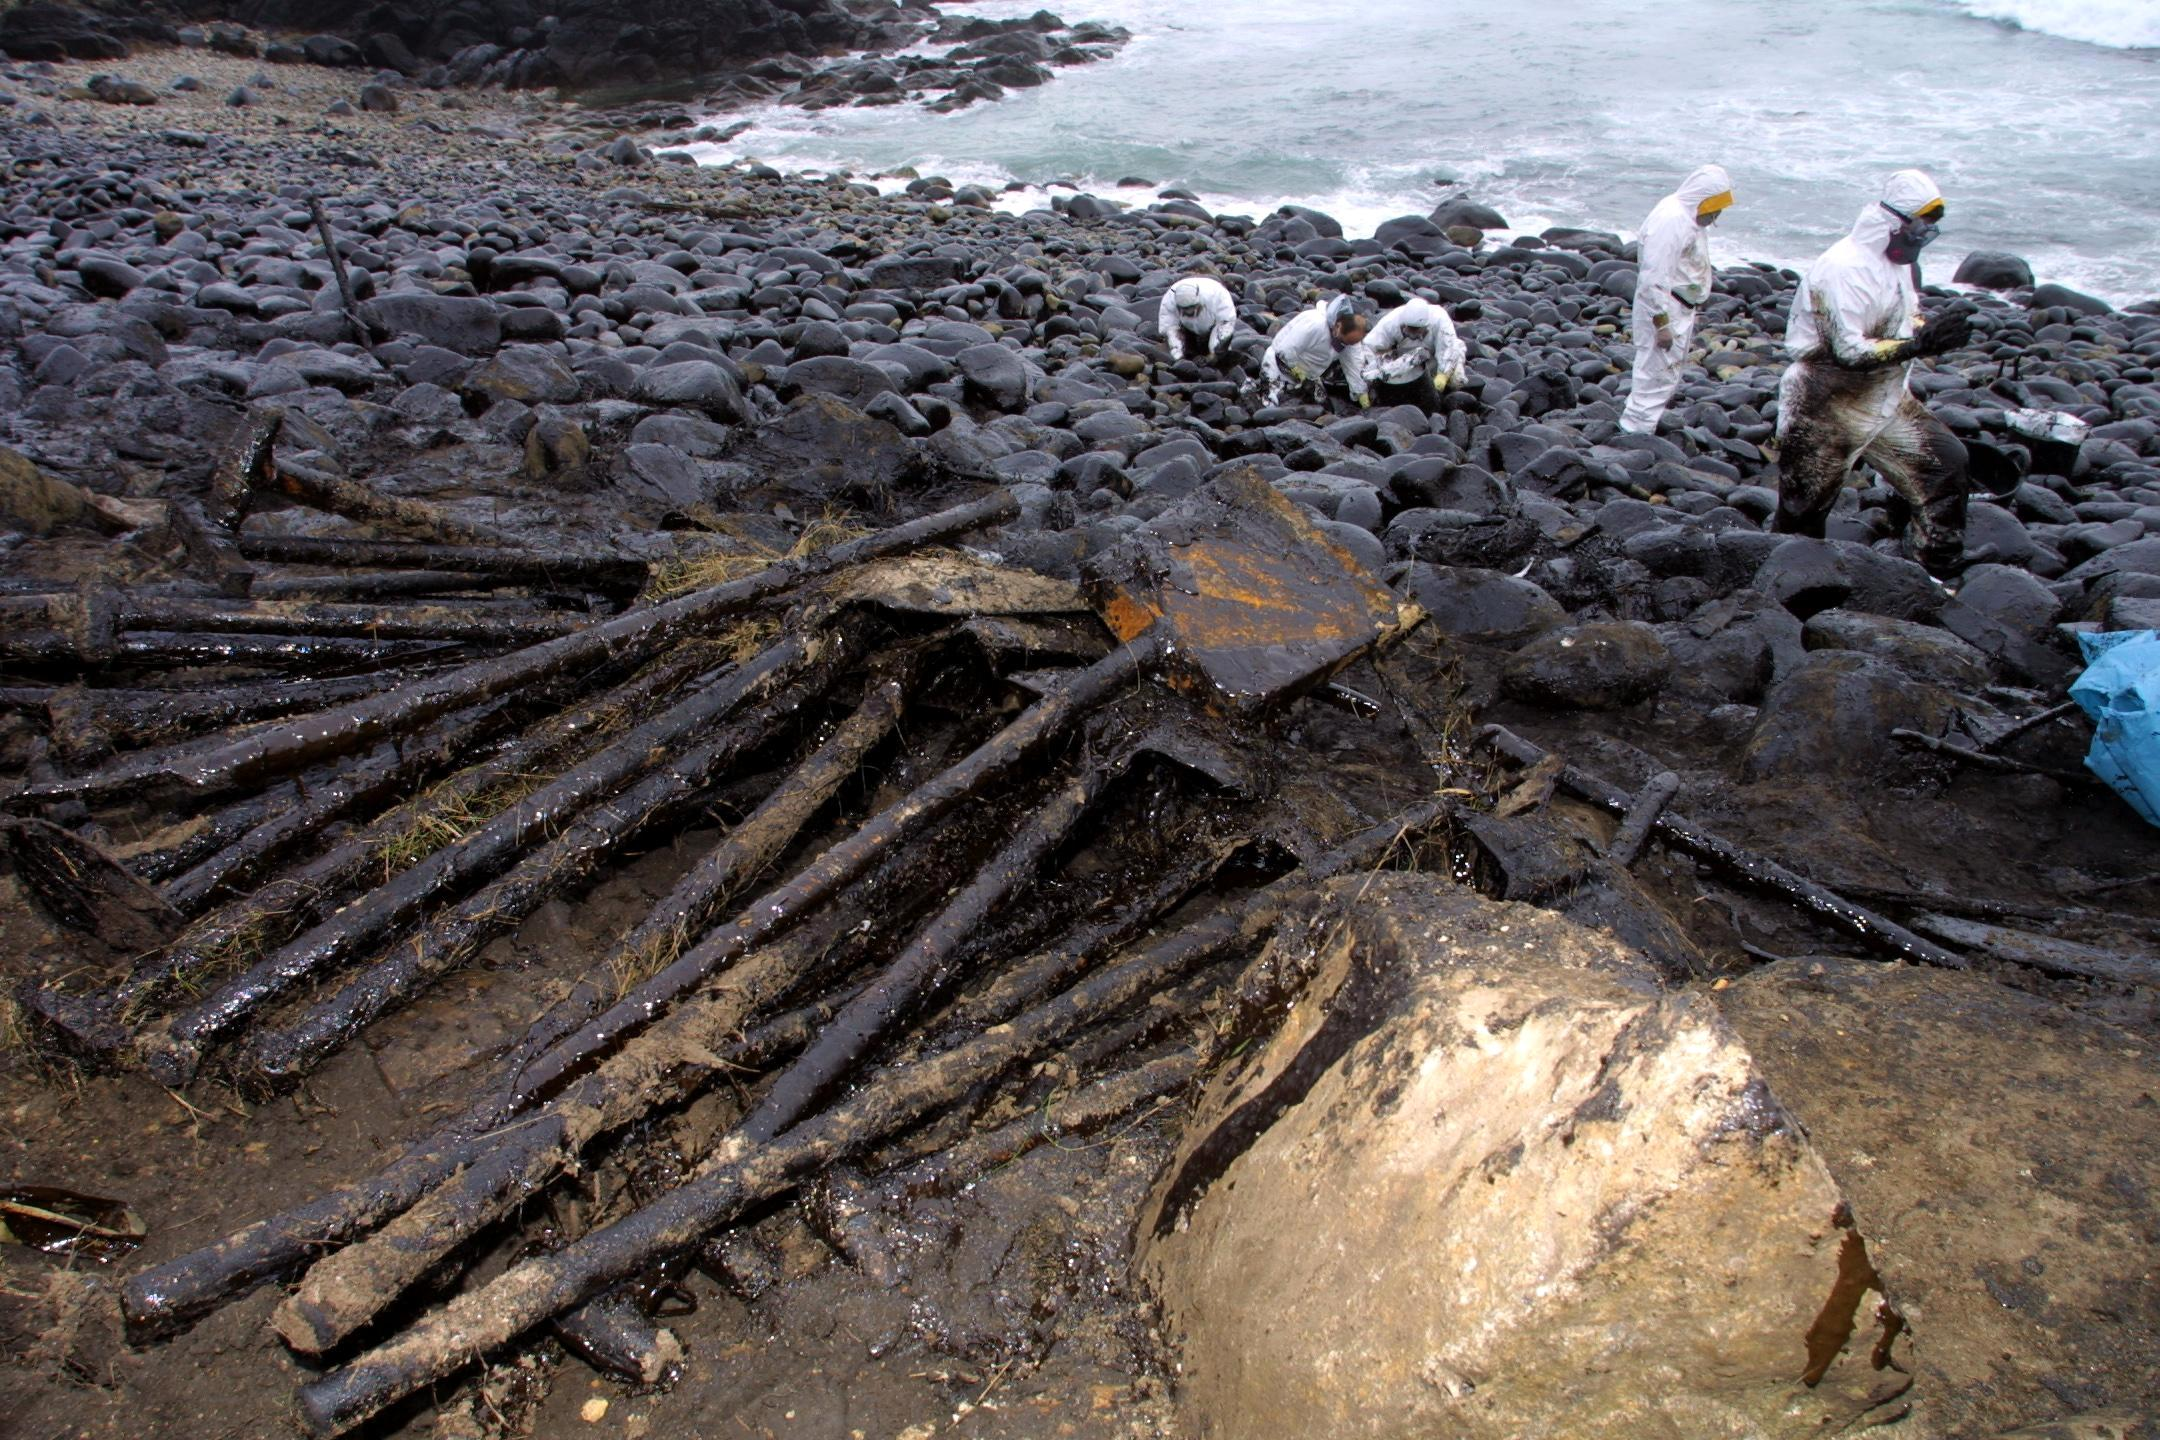
\includegraphics[width=\paperwidth]{images/prestige2.png}}
\begin{frame}{Disaster Scenarios}
\end{frame}
}

\begin{frame}{Losing A Satellite Datacenter}
    \includegraphics[width=\textwidth]{images/lostsatellitedc.png}
\end{frame}

\begin{frame}{Losing A Master Datacenter}
    \includegraphics[width=\textwidth]{images/lostmasterdc.png}
\end{frame}

\begin{frame}{Losing A Master Datacenter}
    \includegraphics[width=\textwidth]{images/lostmasterdchope.png}
\end{frame}

\section{Lessons Learned}

\subsection{Currents Status}
\begin{frame}{Where We Are}
    \begin{itemize}
        \item Using simple buckets on LIVE in one DC
        \item Added relup support for bucket only updates
        \item Hammering SSP using property based testing
        \item Integrating restricted search capabilities
        \item Testing the WAN protocol for inter DC communication
        \item More buckets to go live in H1 2013
        \item Next Master DC coming on H2 2013
    \end{itemize}
\end{frame}

\subsection{Contributions}
% XXX Add Motiejus' basho bench
\begin{frame}{What We've Used}
    \begin{itemize}
        \item Emysql
            \begin{itemize}
                \item (+) multi-database transaction support
                \item (*) multi-timezone support
            \end{itemize}
        \item Eep0018/Jiffy
        \item Estatsd
        \item PropEr
            \begin{itemize}
                \item (*) utf8 generator
            \end{itemize}
        \item Poolboy
        \item Lager
        \item Rebar
            \begin{itemize}
                \item (*) semantic versioning, i.e. [">=1.3.1", "<2.0.0"]
                \item (*) shared dependencies
                \item (*) xref support
            \end{itemize}
        \item Piqi
    \end{itemize}
\end{frame}

\begin{frame}{Questions?}
    \begin{center}
        \includegraphics[width=0.7\textwidth]{images/questions.png}
    \end{center}
\end{frame}

\begin{frame}{That's All Folks!}
    \begin{center}
        \huge{Thanks!}
    \end{center}
\end{frame}

\end{document}

